\chapter{Methods}
\label{methods}
\section{Overview}

In this section we prestent our theoretical methods
and the computation tools used to implement them.

First, in \autoref{md}, we introduce MD generally and describe the two distinct means by 
which the P3HT and ITIC chemistries used in this work were obtained. 
The latter providing a backdrop for an introduction to Planckton in \autoref{planckton}, which
is a conveniece package for performoing MD simulations of OPVs.

In \autoref{marcusmodel}, we present the methods used to chop the
results of the MD simulations into chromophores and calculate the rate of hops between chromophores using the combination of Marcus theory and QCC. 

In \autoref{KMC}, we survey our implementation of the kinetic monte
carlo algorithm for simulating a charge hopping through the chopped up morphology in accordance with its
Marcus rate. 
From there, we show that the 
mean squared displacement across thousands of individual hopping trajectories can provide an accurate charge
mobility prediction in these chemistries.
Finally, in \autoref{morph} the package developed to carry out these simulations is introduced.
 
All the tools used to implement, analyze, and
visualize this work are freely available. 

The packages and tools are enumerated in \autoref{packages}.
\begin{table}[ht]
    \caption{Packages} % title of Table
\centering % used for centering table
\begin{tabular}{|l|p{0.8\linewidth}|} % centered columns (4 columns)
\hline\hline %inserts double horizontal lines
Package/tool & Description \\ [0.5ex] % inserts table
%heading
\hline % inserts single horizontal line
    foyer & python package for applying atom-typing rules  \cite{Klein2018a}\\ [1ex] % inserting body of the table
freud & python package for analyzing particle simulations  \cite{Ramasubramani2020}\\ [1ex] %
HOOMD-blue & general purpuse toolkit for performing simulations.   \cite{Anderson2020a}\\ [1ex] %
    mBuild & python based molecule builder \cite{Klein2018a}\\ [1ex] % [1ex] adds vertical space
MorphCT & python package for simulating and analyzing charge transport from 
    snapshots of MD simulations \cite{jones2017}\cite{cmelab}\\[1ex] 
OVITO basic & tool for visualiztion simulation data \cite{Stukowski2010a}\\[1ex] 
packmol & python package for creating initial configurations of simulations \cite{Martinez2009}\\[1ex] 
Planckton & python based convenience package for running HOOMD-blue
    simulations of OPVs \cite{cmelab}\\[1ex]
Planckton-flow & python based package that supports the use of Planckton on
    high performance clusters\cite{cmelab}\\[1ex]
pySCF & open-source collection of electronic structure modules \cite{Sun2018a}\\[1ex]
signac & python based framework for managing large heterogenous data spaces \cite{Adorf2016}\\[1ex]
VMD & a molecular visualization program for displaying, analyzing, and animating large biomolecular
    systems \cite{Humphrey1996}\\

\hline %inserts single line
\end{tabular}
\label{packages} % is used to refer this table in the text
\end{table}


\section{Molecular Dynamics}
\label{md}
The morphologies used to
obtain the data for this work were obtained from equilibrium Molecular Dynamics simulations. 
Molecular dynamics is a method of computer simulation for predicting the equillibrium geometries of molecular
systems. MD simulations proceed iteratively by solving Newtons laws of motion
in accordance with a predefined interatomic interaction potentials.
At each iteration, the velocities of molecules are
updated based on this solution and they are pushes and pulled in accordance with
the interation between neighbors.

Using the canonical ensemble (NVT), holding the number of
particles, the volume, and the temperature constant allows for the calculation of 
potential energy of the system.  Simulations employ a
Nos\'{e}-Hoover thermostat to maintain the temperature of the simulation. The thermostat in this case keeps
account of the average kinetic temperature, and if it strays too far from the set temperature of the
simulation, it nudges all the velocities in the system up or down, bringing the temperature back into an
acceptable neighborhood of the perscribed simulation temperature \cite{Martyna1994d}\cite{Cao1996}.
The system is considered equilibrated when the potential energy no longer decreases with time. 

We procured the P3HT MD data used in this work off-the-shelf \cite{P3HTData}. This data was provided by
researchers for validation and research purposes \cite{Miller2018}. Using coarse-graining techniques, wherein
molecular segments are unified and treated as individual beads can lower the computational cost and allow for
larger and longer simulations. In this particular case, the researchers ran united-atom simlations, which do
not explicitly keep track of the hydrogens in the simulation, but nevertheless accurately predict equilibrium
geometies. In this case, the fuel for the iterative Newtonian update of positions and velocities 
was the Optimized Potentials for Liquid Simulations United Atom(OPLS-UA) force field.

The ITIC data was generated expressly for use in \autoref{itic}. In the following section we present the
procedure by which it was generated. 

\subsection{MD Software}
\label{planckton}

The ITIC morphology studied in \autoref{itic} was simulated using Plankton-Flow \cite{cmelab} on Fry, 
a high performance computing cluster at Boise State University. 
Planckton-Flow is a dataspace manager that uses
singularity \cite{singularity2017} and docker \cite{Merkel:2014:DLL:2600239.2600241} 
to contanerize a package developed to facilitate simulating self-assembly in
organic photovoltaic materials; Planckton \cite{cmelab}. Docker images are binary files that contain the
entire software stack necessary to execute some code. This allows researchers to minimize dependency issues
and increase reproducibility. However, docker has no native support for the use of GPUs and is not
compatible with the more draconian permissions often present on HPCs. With that, Planckton-flow uses 
Singularity, software designed to overcome these shortcomings,
to pull a docker image of Planckton to a container on the server. 

The forcefield used to generate the ITIC data was the Generalized
Amber Force Field (GAFF)\cite{Wang2004a}.
The Amber forcefield was designed for use in modeling protein and
nucleic acid systems. Serendipitously, the generalized Amber forcefield has parameters for organic molecules
comprised of H,C,N,O, and P and produces accurate simulations of organic molecules for use in OPVs. 

With MD simulations we can predict the self-assembly of OPV materials. To connect the chemistry to the
conductivity of the material we use Marcus theory coupled with KMC.

\section{Marcus Model}
\label{marcusmodel}

Simulation a charge hopping around a morphology requires delineation of
individual chromophores and the estimation of the rate at which a charge will hop to neighboring
chromophores. Each chemistry requires its own justification for which segments in the morphology
can be considered to harbor a fully delocalized charge. Researchers have previously found that, 
despite experimental
results suggesting that delocalizaion occurs along roughly 7 monomers in P3HT, treating every monomer as a
chromophore gives accurate results \cite{jones2017}.
With ITIC, the frontier molecular orbitals, that is, the HOMO
and LUMO have negligible electron density along the side chains. With that, significant computational resources
can be conserved by leaving these atoms out of the of the QCCs. To test this on ITIC, we delineate the
backbone and the whole molecule and compare carrier mobility in \autoref{itic}. 

The rate at which a charge will hop from chromophore $i$ to chromophore $j$, $k_{ij}$,
is estimable by semiclassical Marcus elctron transfer theory and is given by the following equation:
\begin{align}
    k_{ij}  =  |T_{ij}|^2\ \frac{2\pi}{\hbar \sqrt{4 \pi \lambda_{ij} k_{B} T}}\ \exp{\Bigg[ \frac{(\Delta
    E_{ij} - \lambda_{ij})^2}{ 4 \pi \lambda_{ij} k_{B} T} \Bigg] }
    \label{marcus}
\end{align}

with Botzmann's consant, $k_{B}$, and Planck's constant, $\hbar$. The parameters $T_{ij}$, $\lambda_{ij}$,
$\Delta E_{ij}$, $T$ represent the electronic overlap, the reorganization energy, the free energy difference
between chromophores, and
temperature. These are discussed individually in the results section, wherein we test the sensitivity of
the KMC results to these parameters individually.
The accuracy of the Marcus rate is thus dependent on the accuracy with which the inputs can be estimated. In
our work, $\lambda_{ij}$ and $T$ are set as constants. In
the following section we outline our quantum chemical treatment of both $T_{ij}$ and $\Delta E_{ij}$ for all
potential hops throughout the morphology.

\subsection{Quantum Chemical Methods}
Quantum chemistry allows for the estimation of the descrete energy levels of an electron (hole) whose
molecular orbital is implied by the chromophores current atomic configuration.
At the core of Marcus hop rate calculation is the estimation of the energy level of the HOMO (for electron
holes) or LUMO (for electrons). 
The driving force for the reaction, $\Delta E_{ij}$, is the energy offset between chromophore neighbors, which
we approximate as the difference between the HOMO (LUMO) energy level as follows:
\begin{align}
    \Delta E_{ij} = E_{homo, i} - E_{homo, j}.
    \label{gibbs}
\end{align}
The estimation of the electronic orbital overlap between chromophores, $T_{ij}$, is acheived by quantifying
$\Delta E_{ij}$ and comparing that to the difference between the HOMO (LUMO) and HOMO-1 energy levels of a
dimer consisting of the two chromophores. We write this value as follows: $E_{homo,dimer} - E_{homo-1,dimer}$.
This approach is referred to as the energy splitting dimer method
[refs]. An intuiton for why this method works is elusive. However, if we imagine two none interacting
chromophores, quantifying the HOMO of the indivual chromophores is intutive. But what will be the value of the
highest occupied molecular orbital of the dimer, $E_{homo,dimer}$, and the the energy level just below that
energy level, $E_{homo-1,dimer}$?  

With that said, quantum chemical methods give us a framework from which to estimate the homo/lumos. A litany of
methods that use approximations and parameterizations to transform cumbersome ab initio quantum mechanical 
calculations into efficient algorithms for determining the electronic structure of a given compound. Morpcht 
leverages MINDO/3, a variation of the INDO(Intermediate Neglect of Differential Overlap) method,
which is an approximation method that seeks recreate the ab initio Hartree-Fock
results, where the Hatree-Fock theory allows for an iteratively convergent numerical solution to the Shrodinger equation.\cite{Thiel2014}. Calculating electronic structure with this method has
shown good agreement with experimental data and more rigorous Quantum chemical
methods 
\cite{Bredas2002}. Furthermore, variations in TI do not effect mobility calcs
that much (one of evans papers said this).  Results
from the this work compare well to jones2017 which implemented ZINDO/s, another
semi-empirical method. The
previous version of MorphCT utilized ORCA \cite{Neese2012b}to provide the quantum chemical
approximations required to implement
a hopping model of charge transport. Jones2017 showed that with this you can connect MD
provided morphology to charge transport characteristics. A particular 
choice of method comes down to how well we can organize a workflow and integrate the QQC portion of the
workflow modularly. This is because the quantum computational chemistry is a nascent and evolving field of its
own, with quickly increasing efficiencies and accuracies. Therefor, an important consideration is, "how can we
deintigrate and reintigrate a QCC software, tests its efficiency and accuracy, and do it in a way that lays
the groundwork to upgrade or swap it as better options emerge?". 

The software chosen to implement this method is
provided by pySCF (Python-based Simulations of Chemistry Framework) \cite{Sun2018a}. This framework
was chosen in the interest of reproducability and extensibility. PySCF is implemented almost entirly in the Python 
language, which is becoming increasingly ubiquitous in the scientific computing community. Furthermore,
ORCA's proprietary licensing was prohibitive in the efforts to containerize MorphCT for use on cluster and for
creating reproducible results. 

Solving shrodingers equation across tens of thousands of 
chromophores, which will be required to model an OPV material on the order of 10 nm, is untenable. Therefore
justified but drastic simplifications are necessary. Computation of the eigenvalues of the HOMO and HOMO-1
molecular orbitals of the dimer Hamiltonian requires the computation of three integrals: 
the site energy integral, the transfer integral (electronic overlap), and the overlap integral (physical
overlap). Neglecting the latter using an implementation of an INDO method can provide an effective transfer
integral. It is this approximation that allows an estimating of the transfer integral from the calculation of
the dimer splitting energy and the site energy. A further approximation, which is more relevant for highly regular chromopheres is Koopman's
approximation, which further neglects the site energy integral, thereby assuming all chromophores have the same
energetics in isolation.  \cite{Huang2005b}. Other studies have implemented DFT at this stage of predicting
mobility from molecular arrangement to good effect \cite{Deng2004}. However, the P3HT morphologies discussed in the evaluation section of the results
consist of 1000 oligomers of 15 repeating molecular units. 

The upperbound of possible pairwise interactions between chromophose is given by the number of combinations of
$k$ chromophores in a system with $n$ total chromophores is given using `n choose k' notation as follows:
\begin{align}
    {n \choose k} =  \frac{n!}{k!(n-k)!}.
\end{align}

\subsection{Voronoi Analysis}

Now, assigning each molecular unit as a chromophore
gives 15000 indivual QQC calculations and as many as ${15000 \choose 2} = 112,492,500$
dimer QCC calculations. As not all chromophores can be expected to interact electronically,
the latter can be drastically lowered through informed neighborlisting based on spaial proximity as we describe
in the following section. Nevertheless, with the volume of calculations necessary to simulate materials into the
nanometer range, DFT is prohibitively slow. 


A place to mention grits and VMD for chromophore delineation. Having made a choice about where chromoohores
are locatied in the morph we then need to build a neighborlist. 


\begin{figure}
  \center
%\includegraphics[width=25cm]{figures/crystalline_voronoi.png}
  \includegraphics[width=0.99\linewidth]{figures/crystalline_voronoi_smaller.png} 
 % \includegraphics[width=\linewidth]{figures/crystalline_voronoi_smaller.png}
  \caption{2D Voronoi}
  \label{fig:2d}
\end{figure}

 In this workflow neighbor finding is accomplished via
voronoi analysis.
After chopping up the morphology into chromophores, we are required to perform some neighborlisting prior to
QCC. We categorize chromophores as
neihgbors if they share an edge in the voronoi cells around the geometric center of the chromphore. Here, the
cell edges are drawn in a Euclidean way, with lines representing the set of points equidistant from a point
and its geometrically closest neighbor across the line. This analysis takes place in three dimensions. 

As a demonstration, we visualize a 2D voronoi analysis of the crystalline 
P3HT system described in \autoref{md}.
In \autoref{fig:ln}, 15,000 thousand dots represent the single-monomer chromophore's geometric centers projected
in the xy-plane.Here,
a voronoi cell for any given chromophore center is the set of points that are closer to that chromophore
center than any other chromophore center. Euclidean space searching algorithms of
this sort are known to scale with $O(n\log{n})$ in the worst case and as low as $O(n)$ in the average case
\cite{Bentley1980}.
However as can seen from the figure, two points can share cell edges despite being rather far apart. We
therefore, further remove pairs from the neighborlist if they are far enough apart such that it is justifyable
to assume they do not interact electronically enough to effect to charge mobility calculation. This parameter will
depend on the material under investigation as was as the size of the individual chromophores. We tested the
sensitivity of the algorithm to the value (dcut). The figure shows the effect of cutoff distance on value of
calculated mobility. There is a diminishing return on computation around dcut 10. 

Utilizing the freud.locality.Voronoi() 
With a neighbor list built, a single charges movement through the morphology can be simulatied with the
application of a KMC algorthym.

\section{Kinetic Monte Carlo}
\label{KMC}
Taking a charge carrier to be a quasi-particle inserted into a MD generated morpholgy, a KMC
simulation can be run on the bases of the Marcus theory and quantum chemical analysis outlined above. 

With each chromophore taken to be a discrete object, both in python, and with respect to its frontier
molecular orbitals, a charge hopping (transfering) from an excited chromophore to a neighboring chromophore can be modeled
as a discrete event.

Taking \autoref{marcus} to be an
accurate rate of the electron transfer reaction, we implant a charge randomly into the morphology, calculate
the rate of all possible hops(events)
and put them in order of quickest to slowest to form a queue. The hop rate, $k_{ij}$, from the occupied chromophore to any
given neighbering chromophore is taken to be
inversely proportional to the amount of time, $\tau$, that the system will have to wait before that hop will
take place. However, hopping processes at the angstrom level do not proceed deterministically. 
Our implementation, and others like it [NEED REFS?], have
successfully captured the stochasticiity of these systems via a shuffling hopping queue.
The wait time for every potential hop from occupied chromophore $i$ onto a
neighboring chromophore $j$ looks as follows:

\begin{align}
    \tau = \frac{1}{k_{ij}} \cdot \ln{\frac{1}{x}} 
\end{align}
where x is a random number between 0 and 1 and $\log{(1/x)}$ is a scaling factor. To illucidate this
graphically, $\ln{(1/x)}$ is plotted in figure \ref{fig:ln} from 0 to 1. From this we can see that with
a large enough sampling, significant reshuffling of the queue will take place, allowing for a rare hop to jump
the queue.

\begin{figure}
  \center
  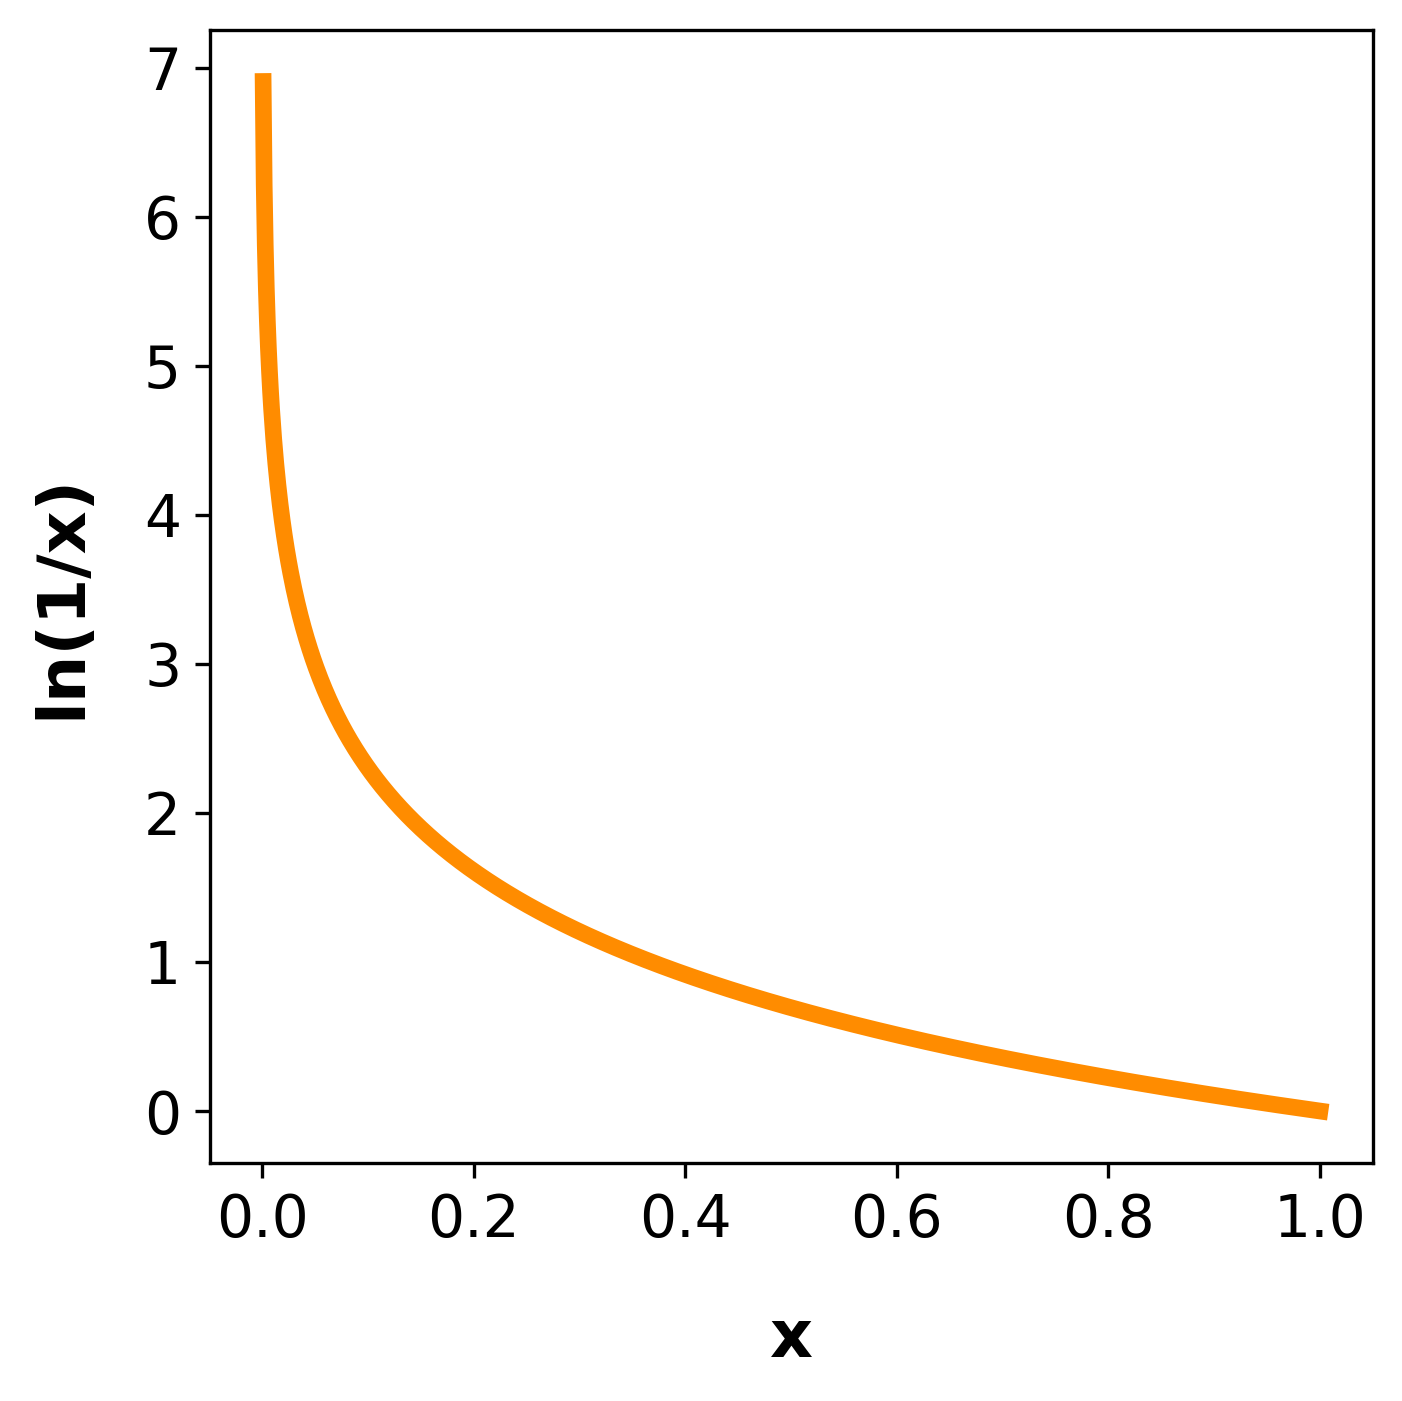
\includegraphics[width=0.8\linewidth]{figures/naturallog.png}
  \caption{Graphical insight into the reshuffling of the wait time queue. Here the x-axis represents the 
    interval from which numbers are drawn randomly such that the wait times in the queue can be scaled 
    by ln(1/x).}
  \label{fig:ln}
\end{figure}

From the rationally shuffled queue, the shortest waittime (quickest available hop) is chosen and the charge is moved to
its new chromophore host. The system is then considered to have moved forward in time by $\tau$. This proceeds
until the charge carrier stalls out or hops past a prespecified lifetime. 



\subsection{KMC analysis}

The choice of carrier lifetimes effectively serve as checkpoints at which the displacement of charge carriers is recorded. For
each specified lifetime, a prescribed number individual KMC simulations is run as described above. When a
given charge carrier hops past the specified lifetime, that is, the addition of the current iterations $\tau$ advances
the simulation beyond the specified lifetime,  its displacement from its starting location is stored in the carrier object. After repeating this over a
statistically significant number of carriers, the carrier data can be aggregated and the mean squared
displacement(MSD) for a particle in the system and that lifetime can be estimated.
It is known that the MSD of a diffusive particle increases linearly as time goes to infinity. 
The slope of the MSD, $D$,  as time
goes to inifinity can be estimated as a linear fit between the MSD's at the specified lifetimes.

There is no objective best practice for determing the slope of the MSD as
time goes to inifinty from simulation data of this kind \cite{Maginn2018}. With that, we seek primarily to simplifiy the MSD analysis as much as
possible so as to accuratley report this stage of the analysis for clarity but also to facilitate apples to
apples comparisons to future works using this workflow. 

Finally, the results of the MSD analysis are then used to determine the zero-field mobility using the following Einstein-Smoluchowski relation:

\begin{align}
    \mu_{0} = \frac{eD}{6k_{B}T},
\end{align}

where $e$ is the elemental charge of a charge carrier, $D$ is the diffusion coefficient, $k_{B}$ is Planck's
constant and $T$ is temperature.  

A benifit to Monte Carlo analysis of this type is that charge carriers can be simultaneously. It is considered
to be "embarrasingly parrel," in that the subprocesses(charge carriers) require no communication.
MorphCT utilizes the python multiprocessing module to divide the prescribed number of charge carriers to be
simulated accross all available cores.  

\subsection{KMC software aka MorphCT}
\label{morph}
MorphCT is developed to facilitate charge characterization of morphological data. It takes GSD files which are
the native file format of the simulation engine HOOMD-blue \cite{Anderson2020a}.
For polymeric materials like P3HT, MorphCT
can identify chromophores with a provided SMILES string. For less regular molecules, explicitly delineating
which atoms belong to which chromophores is required.
%%% Local Variables: 
%%% mode: latex
%%% TeX-master: "BSUmain"
%%% End: 
